\section{Results}

\subsection{Wavelet attenuation: parks damp PM$_{2.5}$ variability}

Across the eight retained 2021 park--outside pairs, attenuation was negative overall, indicating that park interiors consistently reduced PM$_{2.5}$ variability relative to their paired outside comparators. This damping was not uniform across timescales. The strongest attenuation occurred at multi-day scales, with median band-mean attenuation of approximately $-8.0$ dB at 2--7 d and $-7.5$ dB at 7--14 d. Damping was also clearly expressed at sub-diurnal scales, with a median of approximately $-6.3$ dB at 6--18 h. The diurnal band (18--30 h) was the least damped, with a median of approximately $-3.8$ dB. The shortest band (2--6 h) was slightly more negative (about $-4.2$ dB median) but showed greater pair-to-pair variability. Thus, attenuation strengthened from 2--6 h to 6--18 h, dipped at the diurnal band, and then intensified again at multi-day scales. Overall, these results indicate that Bangkok parks buffered PM$_{2.5}$ variability most effectively at sub-diurnal and multi-day timescales, while the daily cycle remained comparatively resistant to damping (Fig.~\ref{fig:attenuation_by_band}).

Substantial heterogeneity was evident across individual parks. At the long-period end, Nong Chok Park showed the strongest attenuation, reaching approximately $-27.4$ dB at 7--14 d, whereas Seri Thai Park showed only weak long-band damping of approximately $-1.9$ dB at the same band. Suan Luang Rama IX Park also showed strong attenuation at daily and multi-day scales, while the three northern-cluster parks paired to Bang Sue District (Chatuchak Park, Wachirabenchathat Park, and Queen Sirikit Park) exhibited consistent broadband negative attenuation of moderate magnitude. In contrast, some parks showed weak or mixed short-band behavior despite remaining clearly damped at longer timescales. This heterogeneity motivated both the regime classification and the explanatory analysis developed below. A representative strong-decoupler example from Nong Chok Park is shown in Fig.~\ref{fig:nongchok_representative_scalograms}, where the park-interior and outside wavelet-power fields can be compared directly across the predefined bands.

\begin{figure}[htbp]
\centering
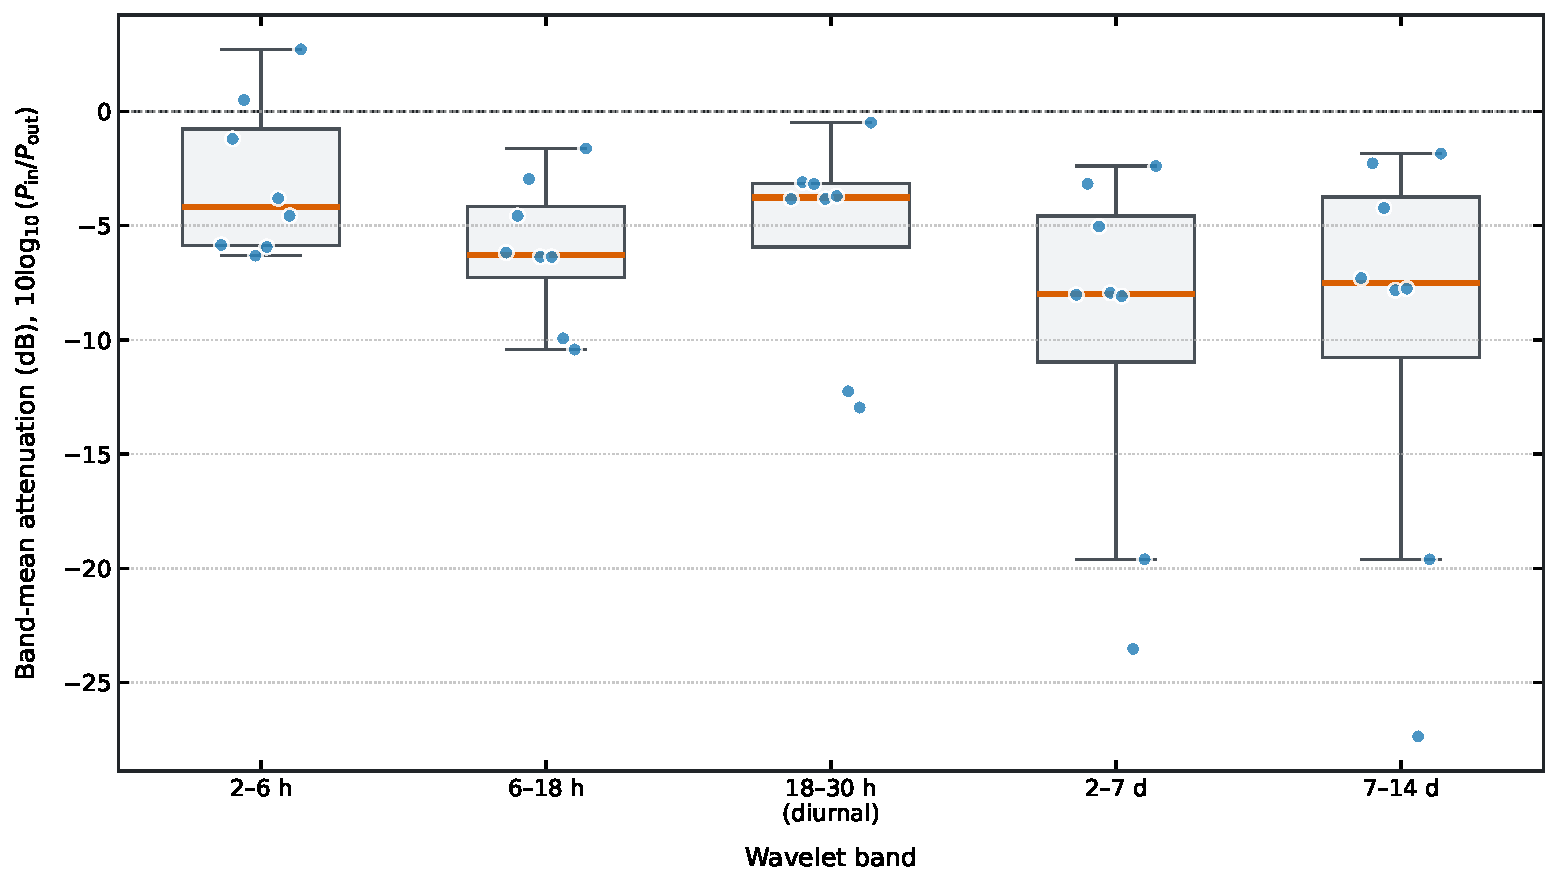
\includegraphics[width=\textwidth]{figures/Fig4_attenuation_by_band_2021.pdf}
\caption{Band-specific attenuation across the eight retained 2021 park--outside pairs. Each point represents one retained pair, while boxplots summarize the distribution within each predefined wavelet band. More negative attenuation values indicate stronger damping of park-interior PM$_{2.5}$ variability relative to the paired outside reference station. The dashed line at 0 dB marks equal variability between park and outside.}
\label{fig:attenuation_by_band}
\end{figure}

\begin{figure}[htbp]
\centering
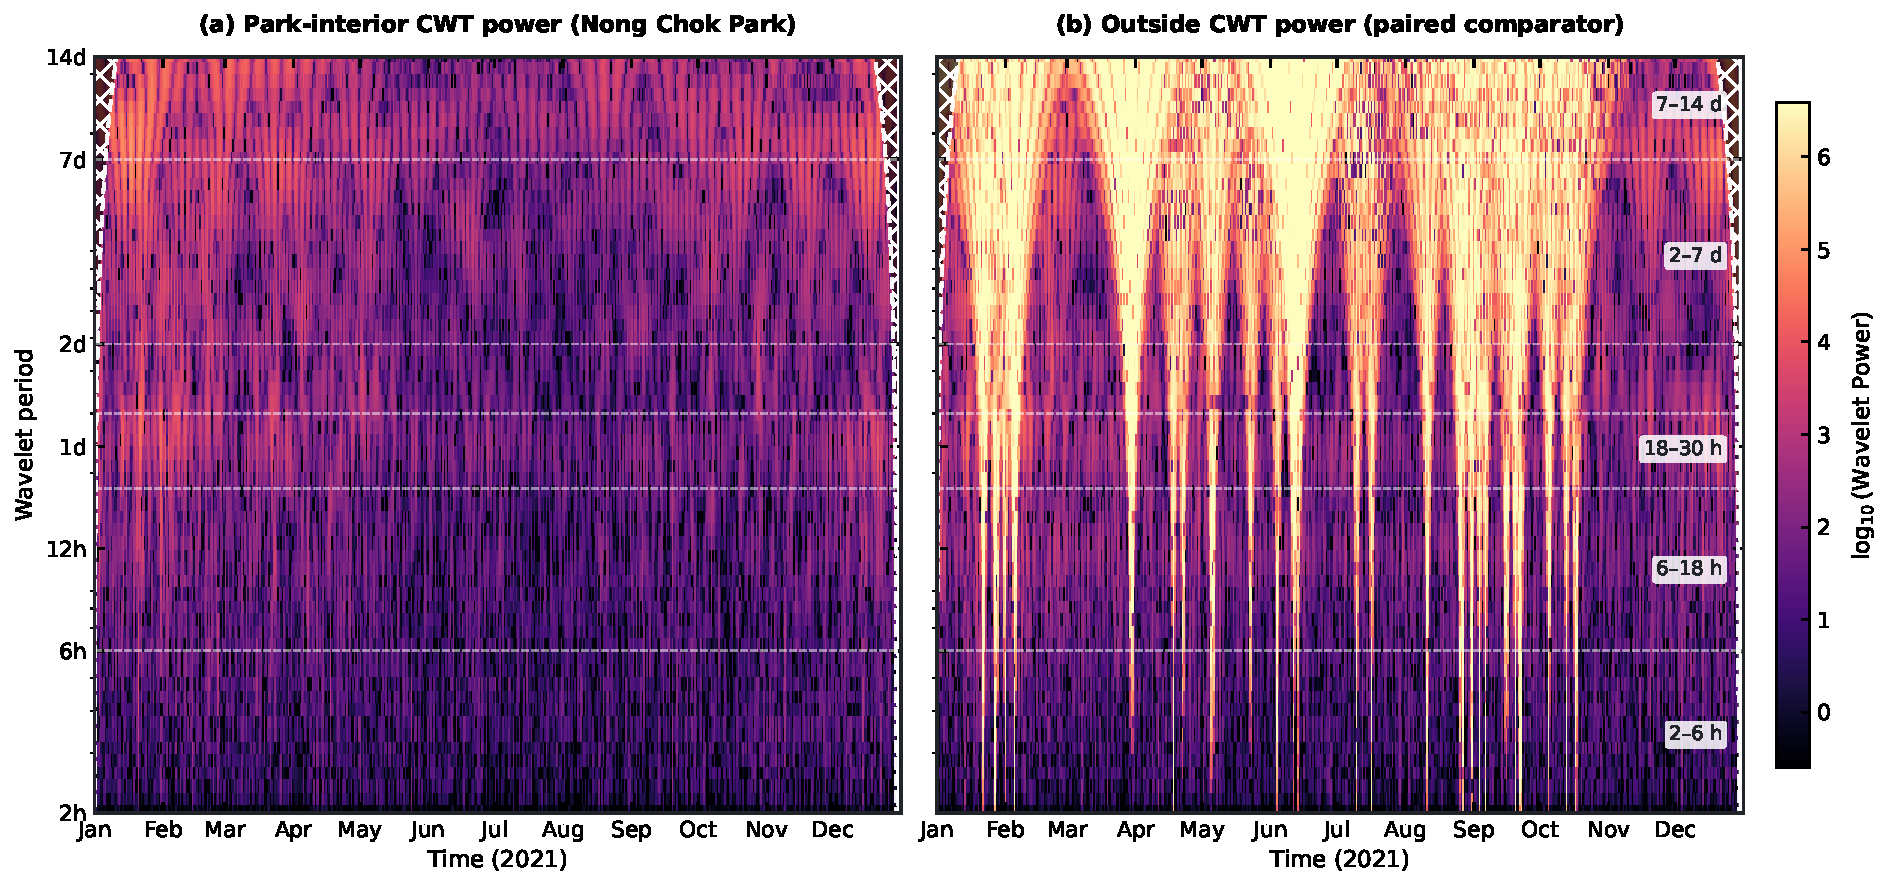
\includegraphics[width=\textwidth]{figures/Fig6_nongchok_representative_scalograms.pdf}
\caption{Representative wavelet-power example for the Nong Chok Park pair, shown here as a strong decoupler. Panel (a) shows park-interior CWT power and panel (b) shows CWT power for the paired outside comparator. Dashed horizontal lines indicate the predefined wavelet-band boundaries used in the main analysis. The hatched region below the dashed cone-of-influence (COI) curve indicates edge-affected areas that should be interpreted cautiously. The COI shown here is the native wavelet COI and therefore extends much farther than the fixed 24-h boundary trim used in the main summaries; long-period sensitivity to this choice was evaluated separately using a stricter 14-day trim.}
\label{fig:nongchok_representative_scalograms}
\end{figure}

\subsection{Wavelet coherence: parks preserve shared urban rhythms}

Wavelet coherence increased markedly from short to longer timescales. Mean coherence was approximately 0.27 at 2--6 h, 0.58 at 6--18 h, 0.78 at the diurnal band, and 0.74 at 2--7 d, before declining to about 0.57 at 7--14 d. Thus, although parks damped PM$_{2.5}$ amplitude, they did not behave as isolated atmospheric islands. Instead, park interiors generally remained embedded within broader city-scale temporal rhythms, especially at the diurnal and 2--7 d bands, with weaker coupling again at 7--14 d (Fig.~\ref{fig:coherence_by_band}).

At short periods, coherence was lower and locally variable, implying that fast fluctuations were more weakly synchronized between parks and their outside comparators than longer-timescale behavior. At diurnal and multi-day scales, coherence became consistently high, with the strongest shared timing evident at the diurnal and 2--7 d bands and lower coherence again at 7--14 d. In other words, Bangkok parks tended to flatten the signal more than they shifted its timing. This remains a more nuanced finding than a simple reduction in mean PM$_{2.5}$ concentration, because it shows that amplitude damping and temporal coupling are related but not identical dimensions of park performance.

\begin{figure}[htbp]
\centering
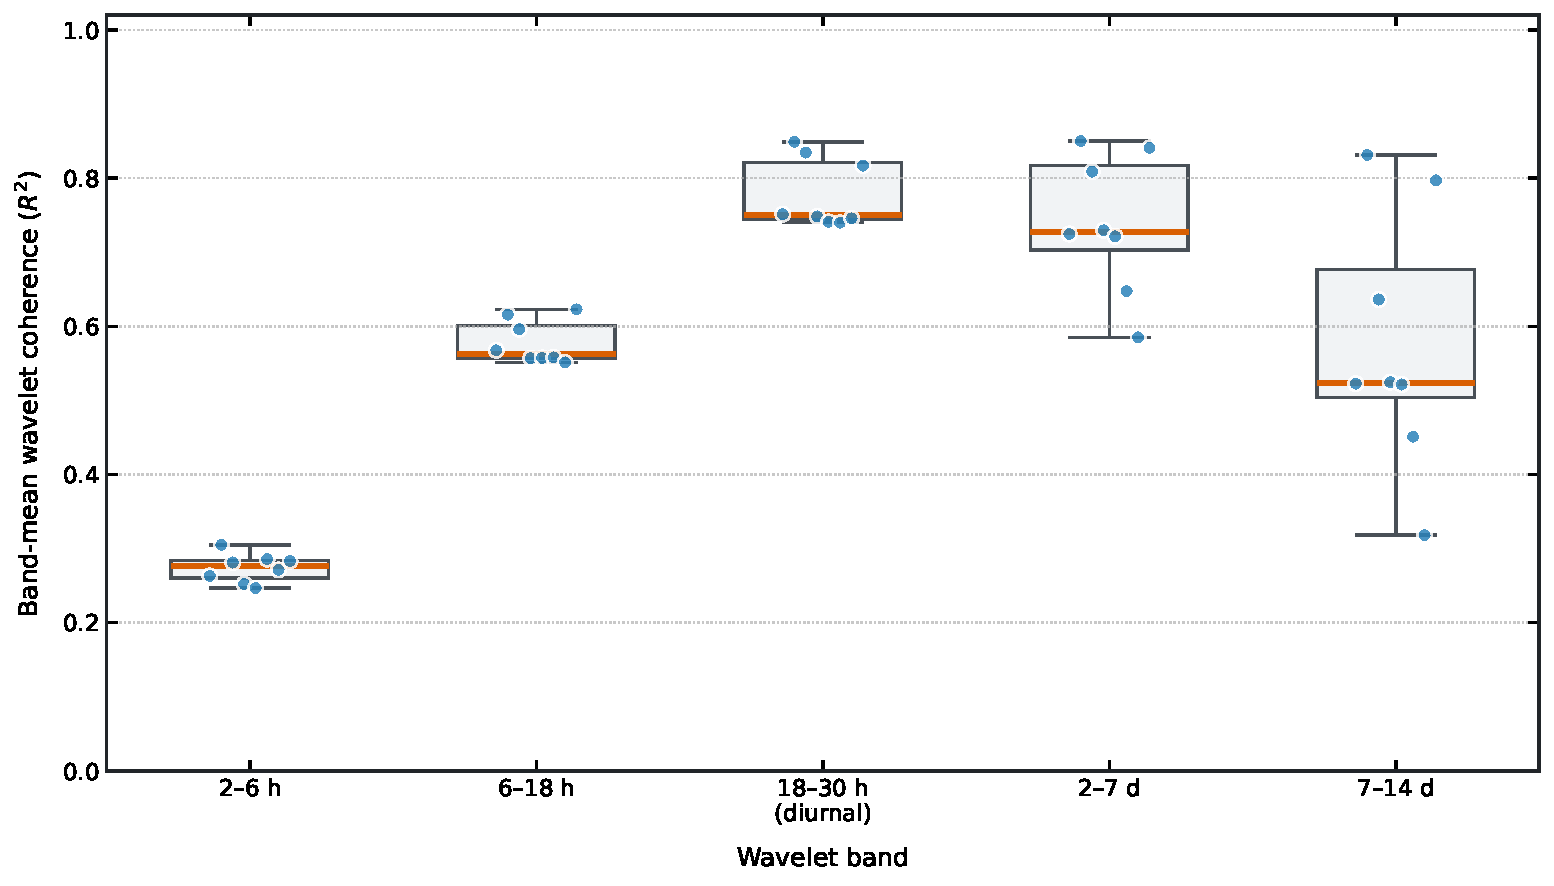
\includegraphics[width=\textwidth]{figures/Fig5_coherence_by_band_2021.pdf}
\caption{Band-specific wavelet coherence across the eight retained 2021 park--outside pairs. Each point represents one retained pair, while boxplots summarize the distribution within each predefined wavelet band. Higher coherence indicates stronger temporal coupling between park-interior and outside PM$_{2.5}$ variability at the corresponding timescale.}
\label{fig:coherence_by_band}
\end{figure}
% [Figure 2C near here: mean attenuation vs. mean coherence for each pair]

\subsection{Three park damping regimes}

When attenuation and coherence were interpreted jointly, the eight retained pairs could be organized into three distinct regimes. The first group comprised \textit{strong decouplers}, represented by Nong Chok Park and Suan Luang Rama IX Park. These parks combined very strong attenuation, especially at daily and multi-day scales, with relatively lower long-band coherence than the rest of the sample. They therefore appeared to damp PM$_{2.5}$ strongly while also partially breaking away from the surrounding urban temporal rhythm.

The second group comprised \textit{moderate broadband dampers}, represented by Chatuchak Park, Wachirabenchathat Park, and Queen Sirikit Park. These parks showed consistently negative attenuation across nearly all bands, but without the extreme long-band decoupling seen in the strongest two cases. Their behavior suggests a more stable, broadband dampening role: they reduced variability across multiple timescales while maintaining moderate synchrony with the outside urban signal.

The third group comprised \textit{weak followers or mixed cases}, represented by Phra Nakhon Park, Lumpini Park, and Seri Thai Park. These parks still showed negative attenuation overall, but their damping was weaker and their coherence remained relatively high, particularly at diurnal and multi-day scales. In practical terms, they tended to follow the outside dynamics more closely than the first two groups. This regime classification is important because it shows that parks within the same city cannot be treated as a single homogeneous class of PM$_{2.5}$ buffers, and the separation of the three groups in mean attenuation--mean coherence space is visualized in Fig.~\ref{fig:regime_scatter}.

A second implication of the regime concept is that park buffering performance should not be interpreted through one scalar summary alone. For example, two parks may have similarly low mean PM$_{2.5}$ but very different temporal signatures: one may act as a strong decoupler that suppresses multi-day peaks, whereas another may simply track the outside station with only modest amplitude reduction. The wavelet framework therefore reveals a hierarchy of buffering behavior that would be obscured by static mean comparisons.

\begin{figure}[htbp]
\centering
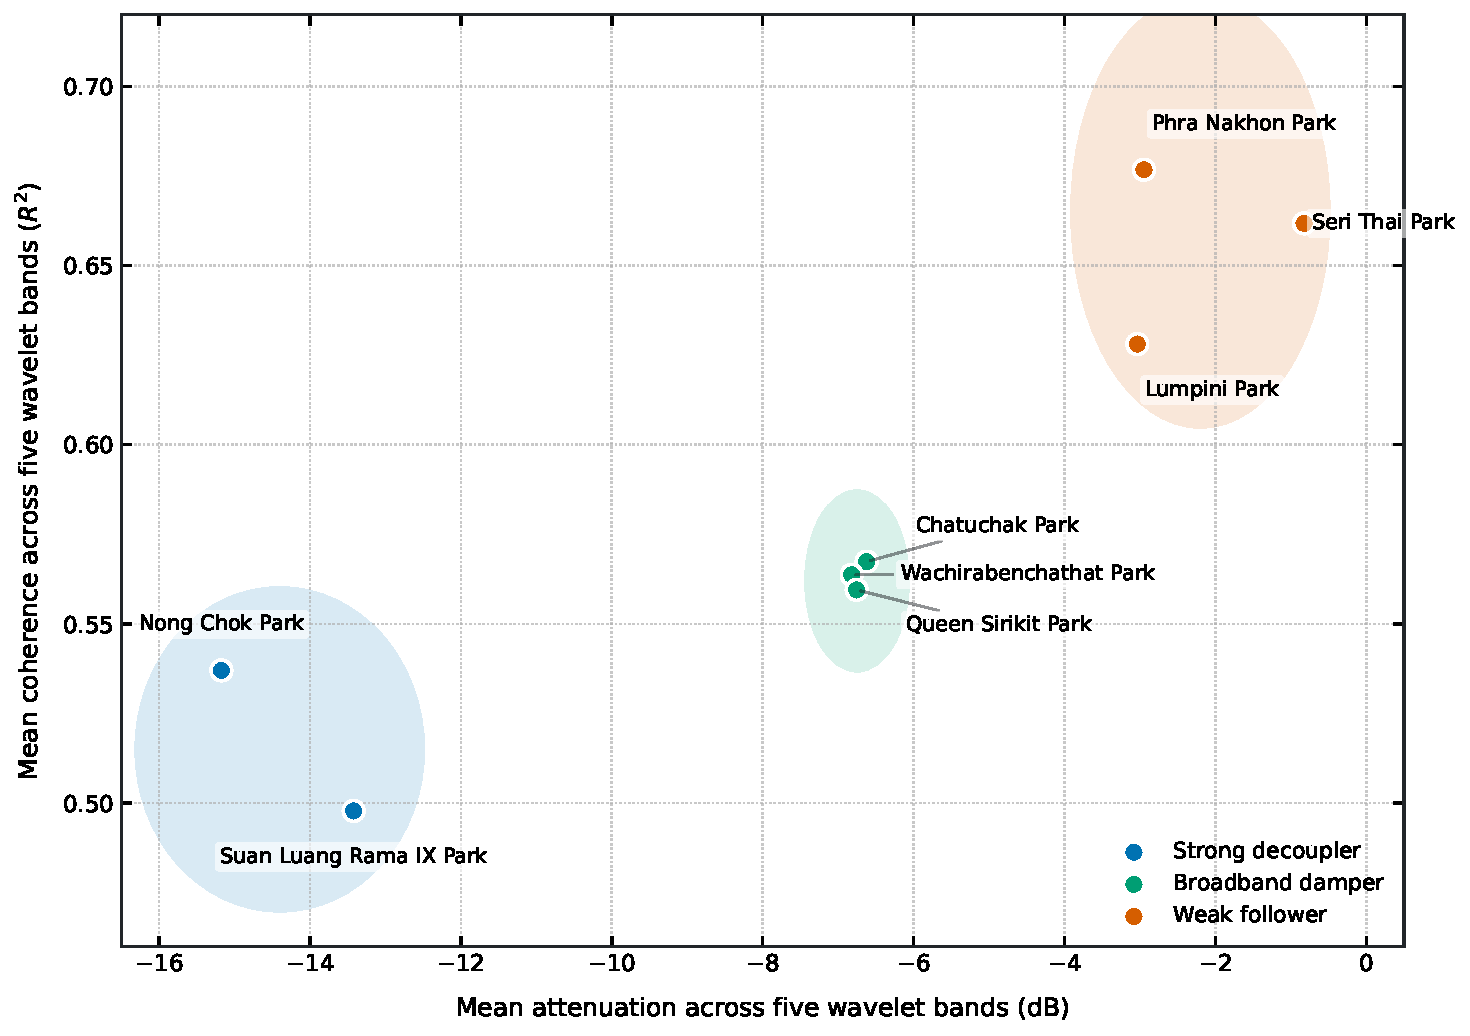
\includegraphics[width=\textwidth]{figures/Fig7_regime_scatter_mean_att_mean_coh.pdf}
\caption{Attenuation--coherence regime map for the eight retained 2021 park--outside pairs, using the mean attenuation and mean coherence aggregated across the five predefined wavelet bands. Each point represents one park pair and is labeled by park name. The shaded groupings indicate the three qualitative regimes identified in the paired wavelet analysis: strong decouplers, broadband dampers, and weak followers.}
\label{fig:regime_scatter}
\end{figure}

Table~\ref{tab:park_regime_summary} summarizes the exact band-mean attenuation and mean coherence values underlying the three-regime classification. Rows are ordered by regime so that the contrast between strong decouplers, moderate broadband dampers, and weak followers or mixed cases can be read directly from the numeric wavelet summaries.

\begin{table}[htbp]
\centering
\caption{Park-level band-mean attenuation and mean wavelet coherence for the eight Tier-A park--outside pairs retained in the 2021 Bangkok analysis. More negative attenuation values indicate stronger damping of park-interior PM$_{2.5}$ fluctuations relative to the paired outside reference station. Row shading indicates the assigned attenuation--coherence regime.}
\label{tab:park_regime_summary}
\begingroup
\setlength{\tabcolsep}{3.2pt}
\renewcommand{\arraystretch}{1.12}
\scriptsize
\resizebox{\textwidth}{!}{%
\begin{tabular}{p{3.9cm}*{10}{c}p{3.8cm}}
\toprule
& \multicolumn{5}{c}{Attenuation (dB)} & \multicolumn{5}{c}{Mean coherence ($R^2$)} & \\
\cmidrule(lr){2-6} \cmidrule(lr){7-11}
Park & 2--6 h & 6--18 h & 18--30 h & 2--7 d & 7--14 d & 2--6 h & 6--18 h & 18--30 h & 2--7 d & 7--14 d & Regime \\
\midrule

\rowcolor{regimedecoupler}
Nong Chok Park
& -3.806 & -9.936 & -12.254 & -23.529 & -27.362
& 0.29 & 0.56 & 0.74 & 0.65 & 0.45
& Strong decoupler \\

\rowcolor{regimedecoupler}
Suan Luang Rama IX Park
& -4.571 & -10.424 & -12.962 & -19.607 & -19.611
& 0.27 & 0.55 & 0.75 & 0.59 & 0.32
& Strong decoupler \\

\rowcolor{regimebroadband}
Chatuchak Park
& -5.846 & -6.179 & -3.834 & -8.026 & -7.296
& 0.26 & 0.57 & 0.75 & 0.72 & 0.52
& Moderate broadband damper \\

\rowcolor{regimebroadband}
Wachirabenchathat Park
& -6.314 & -6.365 & -3.832 & -7.941 & -7.829
& 0.25 & 0.56 & 0.75 & 0.73 & 0.52
& Moderate broadband damper \\

\rowcolor{regimebroadband}
Queen Sirikit Park
& -5.936 & -6.371 & -3.708 & -8.085 & -7.758
& 0.25 & 0.56 & 0.74 & 0.72 & 0.52
& Moderate broadband damper \\

\rowcolor{regimeweak}
Phra Nakhon Park
& -1.203 & -4.572 & -3.101 & -3.169 & -2.276
& 0.31 & 0.62 & 0.85 & 0.85 & 0.83
& Weak follower / mixed case \\

\rowcolor{regimeweak}
Lumpini Park
& 0.501 & -2.956 & -3.176 & -5.037 & -4.226
& 0.28 & 0.60 & 0.83 & 0.81 & 0.64
& Weak follower / mixed case \\

\rowcolor{regimeweak}
Seri Thai Park
& 2.713 & -1.623 & -0.489 & -2.396 & -1.850
& 0.28 & 0.62 & 0.82 & 0.84 & 0.80
& Weak follower / mixed case \\

\bottomrule
\end{tabular}%
}
\endgroup
\end{table}

% [Figure 3 near here: representative peak-flattening time-series example]

\subsection{Mean land-cover contrast provides a first-order explanation}

The first explanatory layer considered whether simple park--outside land-cover contrasts based on mean Sentinel-2 buffer summaries were associated with the observed wavelet outcomes. The strongest simple-buffer relationship was a positive association between $\Delta$NDBI at the 250 m scale and 6--18 h attenuation, with Spearman $\rho = 0.595$ ($p = 0.120$). Because both $\Delta$NDBI and attenuation can take negative values in this dataset, this positive rank association means that more negative park--outside built-up contrast was associated with more negative attenuation, that is, stronger damping. An equally strong long-band built-up signal also appeared at the 500 m scale, where $\Delta$NDBI was positively associated with 7--14 d attenuation ($\rho = 0.595$, $p = 0.120$). The strongest greenness-based mean-buffer signal was a negative association between $\Delta$NDVI at the 500 m scale and 7--14 d attenuation, with $\rho = -0.571$ ($p = 0.139$). These top mean-buffer relationships are visualized in Fig.~\ref{fig:mean_buffer_landcover_scatter}.

\begin{figure}[htbp]
\centering
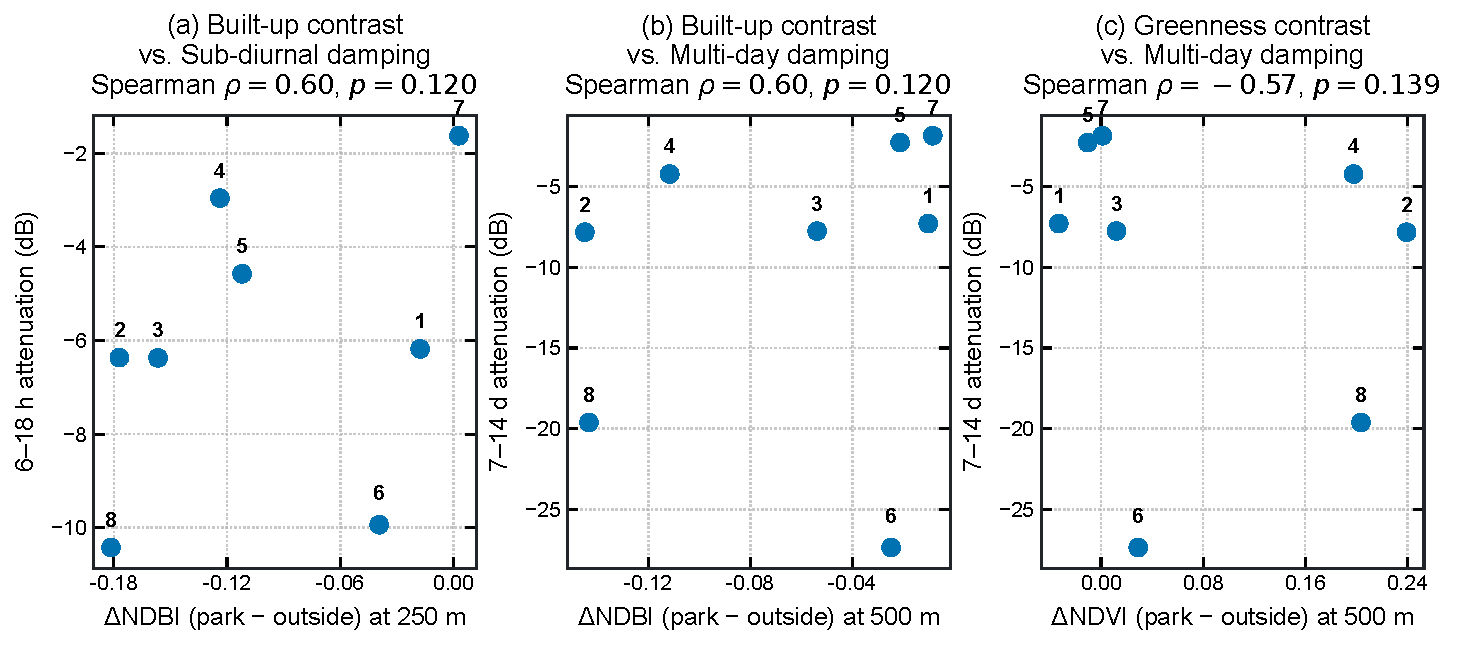
\includegraphics[width=\textwidth]{figures/Fig8_top_mean_buffer_landcover_relationships_2021.pdf}
\caption{Top mean-buffer land-cover relationships between park--outside contrasts and wavelet attenuation outcomes across the eight retained 2021 pairs.
Panels show the strongest mean-buffer associations emphasized in the Results: (i) $\Delta$NDBI at 250 m versus 6--18 h attenuation, (ii) $\Delta$NDBI at 500 m versus 7--14 d attenuation, and (iii) $\Delta$NDVI at 500 m versus 7--14 d attenuation.
Each point is one retained park--outside pair, labeled numerically as follows: 1 = Chatuchak Park (Bang Sue), 2 = Wachirabenchathat Park (Bang Sue), 3 = Queen Sirikit Park (Bang Sue), 4 = Lumpini Park (Pathum Wan), 5 = Phra Nakhon Park (Lat Krabang), 6 = Nong Chok Park (Nong Chok), 7 = Seri Thai Park (Bueng Kum), and 8 = Suan Luang Rama IX (Prawet).}
\label{fig:mean_buffer_landcover_scatter}
\end{figure}

These relationships remained directionally stable under leave-one-out testing.
For 250 m $\Delta$NDBI versus 6--18 h attenuation, the correlation remained positive across all leave-one-out subsets, ranging from $\rho = 0.393$ to $\rho = 0.821$.
For 500 m $\Delta$NDBI versus 7--14 d attenuation, the leave-one-out correlations also remained positive, ranging from $\rho = 0.393$ to $\rho = 0.786$.
For 500 m $\Delta$NDVI versus 7--14 d attenuation, the correlation remained negative throughout, ranging from $\rho = -0.714$ to $\rho = -0.464$.
Thus, although the sample size was small and the p-values should be interpreted cautiously, the sign consistency indicates that these first-order relationships were directionally robust and not solely dependent on any single park--outside pair, even though their strength varied across leave-one-out subsets.
These leave-one-out results are summarized in Fig.~\ref{fig:loo_robustness_mean_buffer}.

\begin{figure}[htbp]
\centering
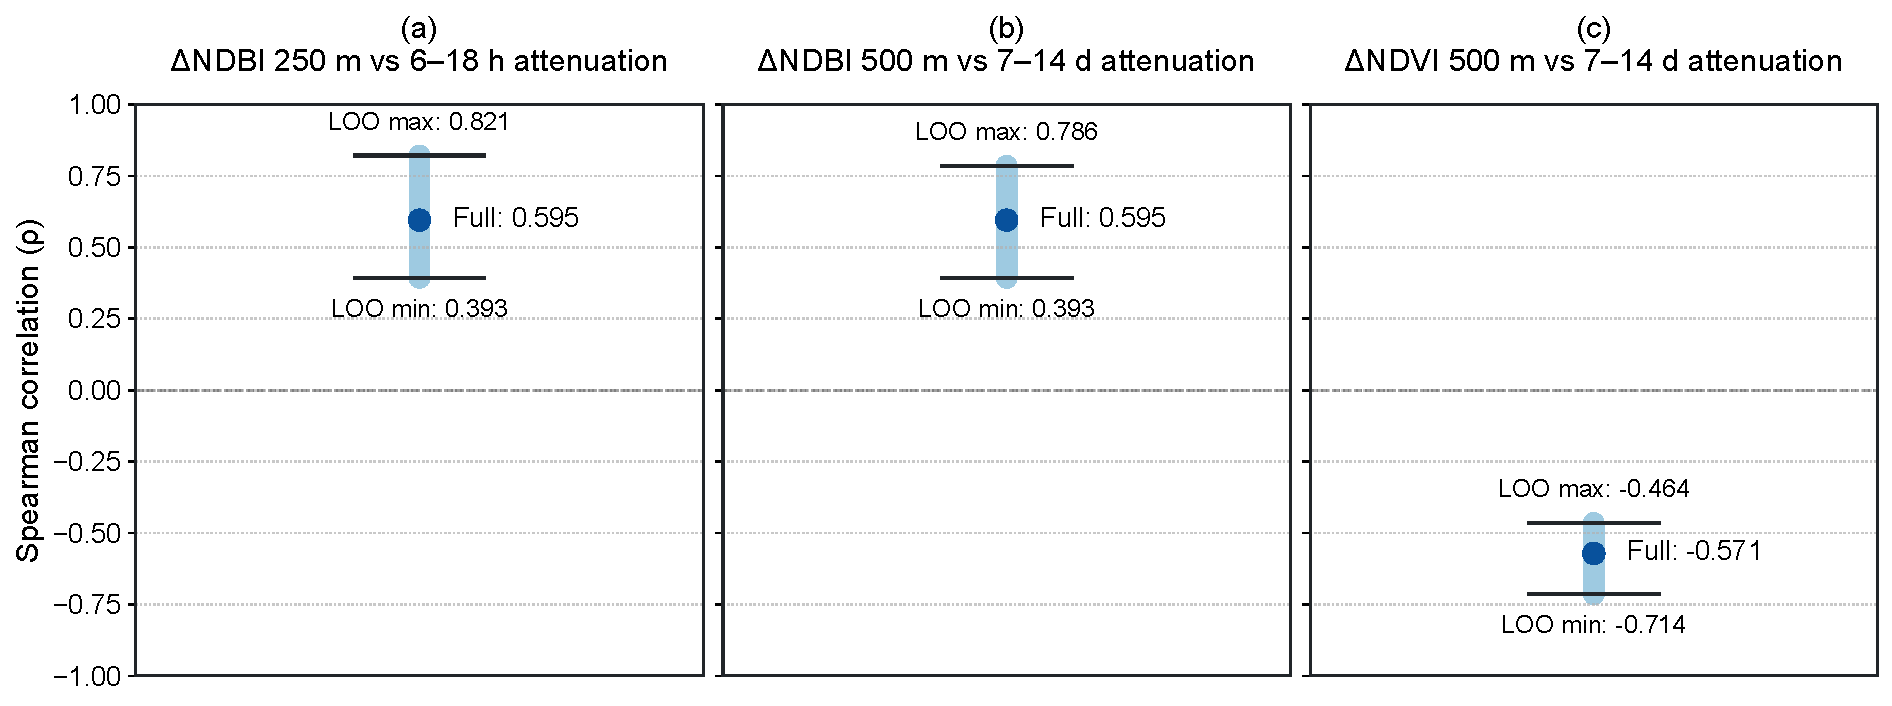
\includegraphics[width=\textwidth]{figures/Fig9_loo_robustness_mean_buffer_relationships_2021.pdf}
\caption{Leave-one-out robustness of the three leading mean-buffer land-cover relationships emphasized in the Results.
In each panel, the dark point shows the full-sample Spearman $\rho$ for the complete eight-pair dataset, while the vertical range shows the minimum and maximum $\rho$ obtained across all leave-one-out subsets.
Each leave-one-out subset contains $n=7$ pairs, obtained by dropping one park--outside pair at a time from the full eight-pair dataset.
Sign consistency across the full-sample and leave-one-out estimates indicates that the leading mean-buffer relationships are directionally robust to omission of any single pair.}
\label{fig:loo_robustness_mean_buffer}
\end{figure}

Taken together, the mean-buffer layer suggests a coherent first-order pattern: stronger park--outside built-up contrast tended to be associated with stronger attenuation, while stronger park--outside greenness contrast tended to be associated with stronger long-band damping in the opposite direction of the built-up effect.
However, these average contrasts were not sufficient to explain the full hierarchy of park behavior.
Nong Chok Park, for example, showed exceptionally strong damping without being reducible to a single mean greenness metric, while some greener parks still behaved as weaker followers.
This indicated that mean NDVI and NDBI were useful first-order descriptors, but not a complete explanatory framework on their own.

\subsection{Ring-gradient land-cover structure strengthens the explanation}

The annulus-based analysis substantially sharpened the land-cover interpretation by moving beyond cumulative mean buffers toward radial structure. In this layer, the strongest signals appeared most clearly for coherence, especially at short timescales. The contrast between the core and outer ring in outside-site NDVI showed a strong negative association with 2--6 h coherence ($\rho = -0.756$, $p = 0.030$) and with 6--18 h coherence ($\rho = -0.756$, $p = 0.030$). Conversely, the contrast between the core and outer ring in outside-site NDBI showed a strong positive association with 2--6 h coherence ($\rho = 0.708$, $p = 0.050$) and with 6--18 h coherence ($\rho = 0.708$, $p = 0.050$), with a similar but slightly weaker signal for diurnal coherence ($\rho = 0.683$, $p = 0.062$). The identical correlation values across the 2--6 h and 6--18 h bands reflect the same rank ordering of the eight retained pairs across those two coherence metrics in this small sample.

These results indicate that the radial organization around the outside comparator site mattered strongly for short-band synchrony. When the outside-site core was greener relative to its outer ring, short-band park--outside coherence tended to be lower; when the outside-site core was more built-up relative to its outer ring, short-band coherence tended to be higher. In other words, the local spatial structure of the comparator environment influenced how tightly parks remained synchronized with nearby urban fluctuations. %The strongest annulus-based relationships are visualized in Fig.~\ref{fig:annulus_ring_gradient} and summarized numerically in Table~\ref{tab:annulus_top_correlations}.

The annulus analysis also contributed to the attenuation interpretation, although these signals were somewhat weaker than the coherence results. Park--outside built-up contrast in the 250--500 m ring was positively associated with 7--14 d attenuation ($\rho = 0.619$, $p = 0.102$), while the related mid-ring built-up advantage metric showed the corresponding negative association ($\rho = -0.619$, $p = 0.102$). Similar though slightly weaker patterns appeared for long-band coherence. Taken together, these results support the idea that green-core advantage, built-edge pressure, and contrast persistence provide a better explanation of park buffering behavior than simple average greenness alone.

A key implication is that park performance was relational rather than purely internal. The strongest spatial signals were not limited to the park itself; they also depended on the radial structure of the outside comparator site. This is a central result of the study: PM$_{2.5}$ damping by parks depends not only on whether a park is green, but also on how the surrounding urban landscape is organized around both members of the pair.

\begin{figure}[htbp]
\centering
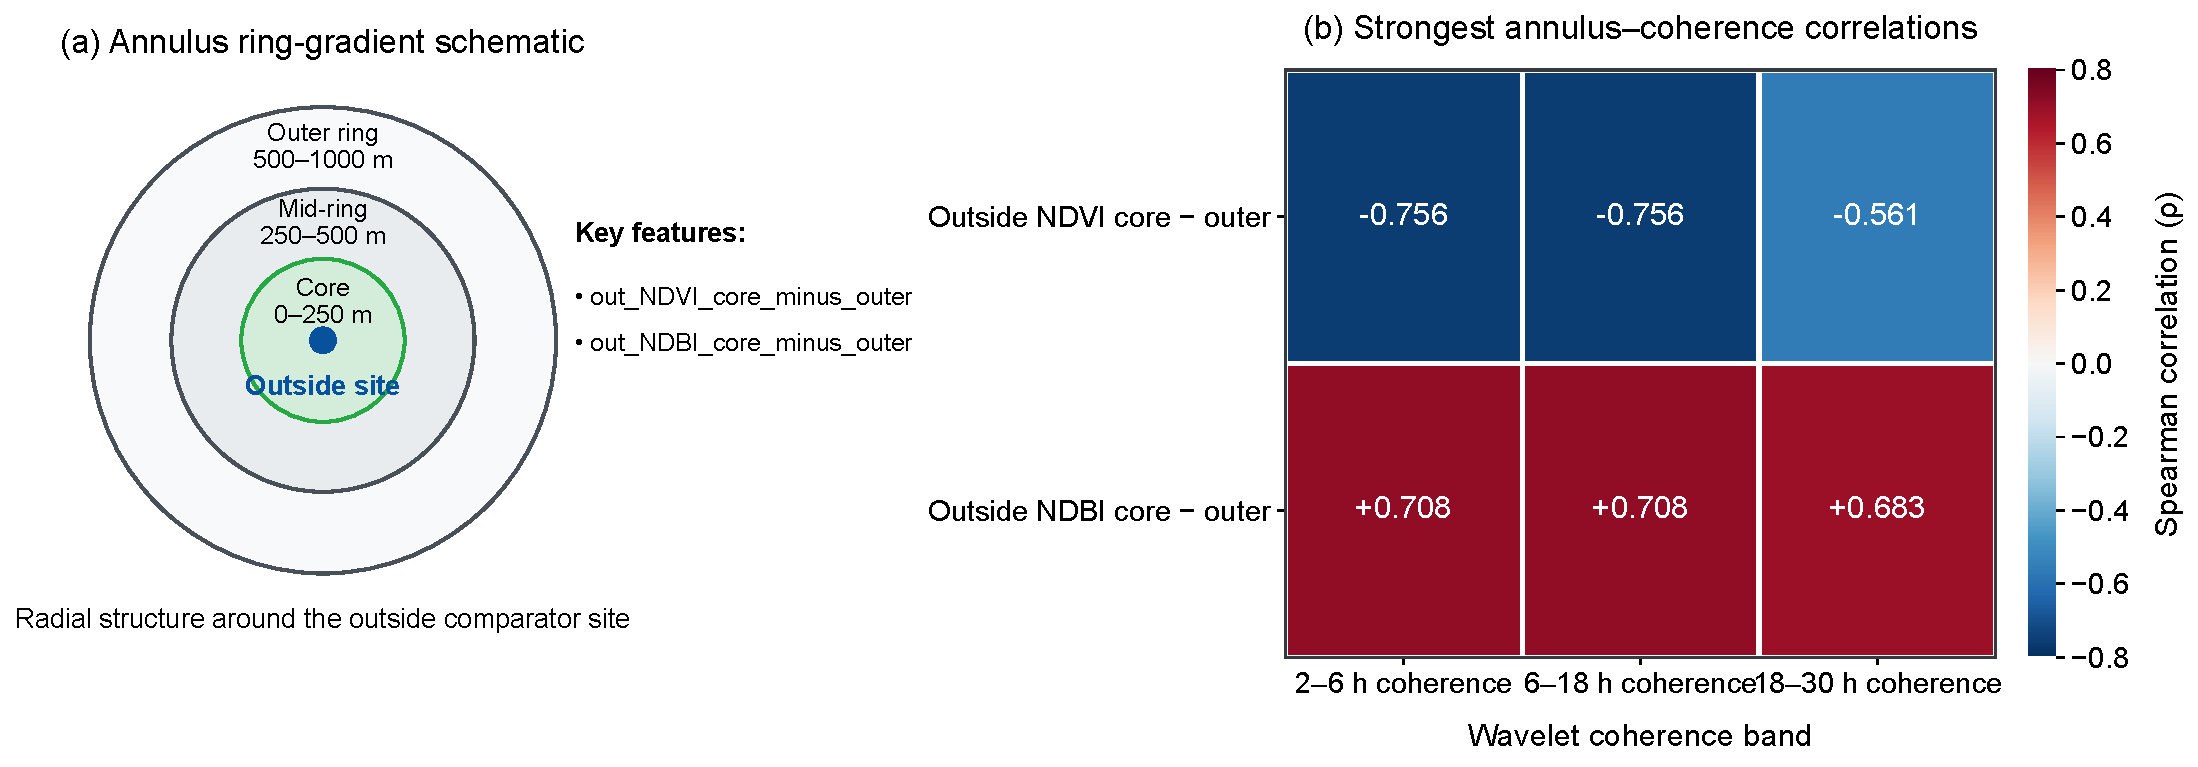
\includegraphics[width=\textwidth]{figures/Fig10_annulus_ring_gradient_schematic_results_2021}
\caption{Annulus-based ring-gradient interpretation of the strongest outside-site land-cover structure signals across the eight retained 2021 park--outside pairs. (a) Schematic of the annulus framework around the outside comparator site, showing the core (0--250 m), mid-ring (250--500 m), and outer ring (500--1000 m). The key gradients emphasized here are the core-minus-outer contrasts for outside-site NDVI and NDBI. (b) Spearman correlations between these outside-site core-minus-outer annulus contrasts and wavelet coherence bands. Outside-site NDVI core minus outer ring showed strong negative associations with 2--6 h coherence ($\rho = -0.756$), 6--18 h coherence ($\rho = -0.756$), and weaker negative association with 18--30 h coherence ($\rho = -0.561$). Outside-site NDBI core minus outer ring showed strong positive associations with 2--6 h coherence ($\rho = 0.708$), 6--18 h coherence ($\rho = 0.708$), and 18--30 h coherence ($\rho = 0.683$). These results indicate that greener outside-site cores relative to their outer rings tended to reduce short-band park--outside synchrony, whereas more built-up outside-site cores tended to increase it. Identical $\rho$ values for the 2--6 h and 6--18 h bands reflect identical rank orderings across pairs, not a tabulation error.}
\label{fig:annulus_ring_gradient}
\end{figure}

% \begin{table}[htbp]
% \centering
% \caption{Strongest annulus-based relationships between radial land-cover structure and wavelet outcomes across the eight retained 2021 park--outside pairs. Correlations are ranked by absolute Spearman $\rho$ among the strongest nonredundant band-specific relationships emphasized in the annulus analysis. Positive $\rho$ indicates that larger annulus-feature values are associated with larger wavelet-response values; negative $\rho$ indicates the opposite. Identical $\rho$ values for the 2--6 h and 6--18 h coherence bands reflect identical rank orderings across pairs, not a tabulation error.}

% \label{tab:annulus_top_correlations}
% \begingroup
% \setlength{\tabcolsep}{4pt}
% \renewcommand{\arraystretch}{1.12}
% \scriptsize
% \begin{tabular}{p{6.0cm}p{3.0cm}cc}
% \toprule
% Annulus feature & Wavelet response & Spearman $\rho$ & $p$-value \\
% \midrule
% Outside-site NDVI core minus outer ring & Coherence (2--6 h) & $-0.756$ & 0.030 \\
% Outside-site NDVI core minus outer ring & Coherence (6--18 h) & $-0.756$ & 0.030 \\
% Outside-site NDBI core minus outer ring & Coherence (2--6 h) & $+0.708$ & 0.050 \\
% Outside-site NDBI core minus outer ring & Coherence (6--18 h) & $+0.708$ & 0.050 \\
% Outside-site NDBI core minus outer ring & Coherence (18--30 h) & $+0.683$ & 0.062 \\
% Park--outside $\Delta$NDBI in the 250--500 m ring & Attenuation (7--14~d) & $+0.619$ & 0.102 \\
% Built mid-ring advantage & Attenuation (7--14 d) & $-0.619$ & 0.102 \\
% \bottomrule
% \end{tabular}
% \endgroup
% \end{table}

\subsection{Water-related metrics add a targeted coherence signal}

The water-related feature layer added a strong but more targeted explanatory component. The clearest signals again appeared for short-band and 6--18 h coherence. Park--outside contrast in mid-ring water fraction relative to the outer ring showed the strongest coherence relationship in the full water scan, with $\rho = 0.810$ and $p = 0.015$ for both 6--18 h coherence and the aggregated short-band coherence metric. The contrast between the core and outer ring in outside-site NDWI and the corresponding contrast in outside-site MNDWI also showed strong positive associations with 2--6 h coherence and 6--18 h coherence (both $\rho = 0.756$, $p = 0.030$). In addition, the contrast between the core and outer ring in outside-site MNDWI showed a strong positive association with 2--6 h attenuation ($\rho = 0.805$, $p = 0.016$).

These results suggest that surface-water context and moisture-related radial structure were especially relevant to short-timescale coupling rather than to broadband long-period damping. In practical terms, water metrics helped explain whether the park and outside station behaved more synchronously at fast and sub-diurnal timescales, rather than serving as a dominant predictor of multi-day attenuation. This is consistent with a microenvironmental interpretation, in which moisture-sensitive land-cover structure may modulate local short-timescale dynamics more directly than it controls broader episode-scale buffering. The leading water-context coherence relationships are visualized in Fig.~\ref{fig:water_context_coherence}.

\begin{figure}[htbp]
\centering
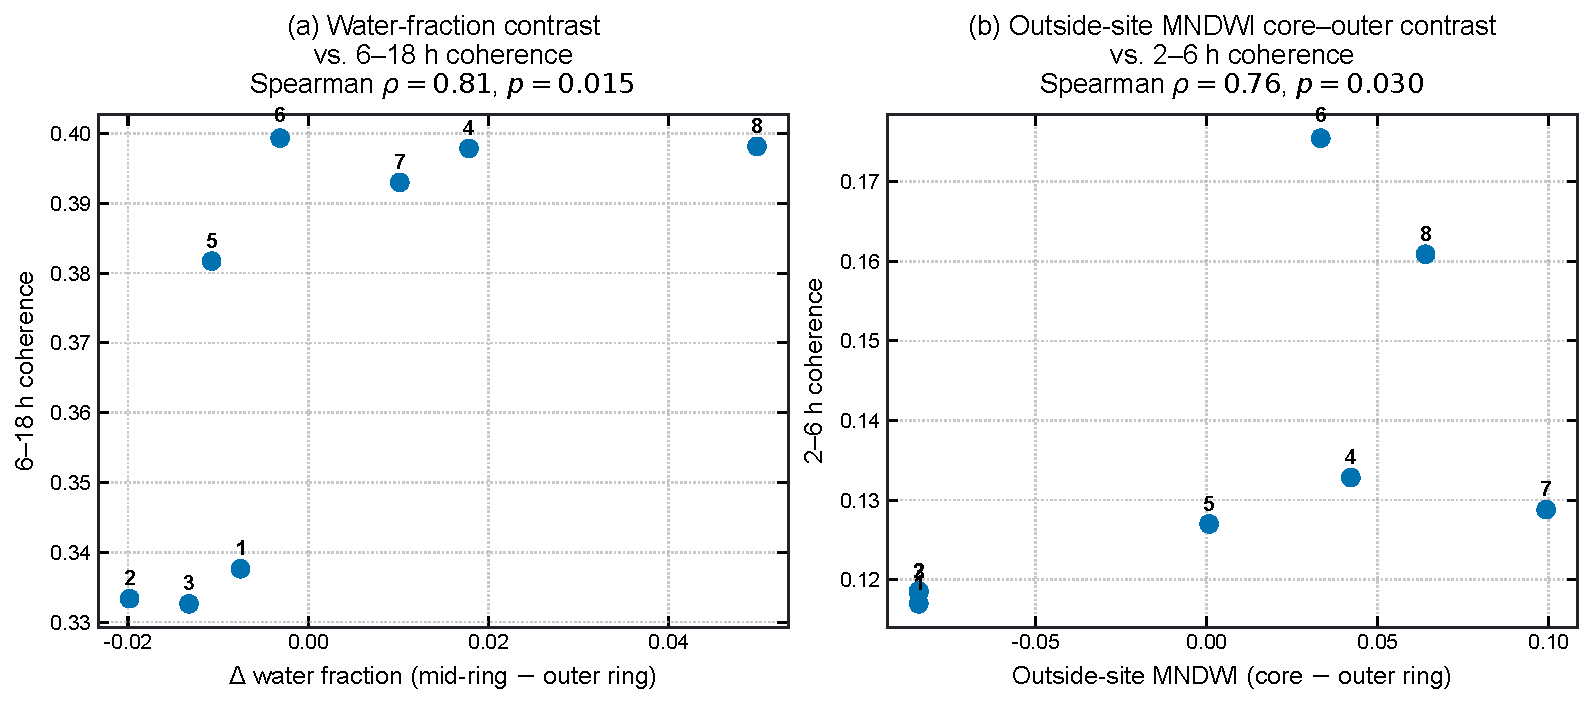
\includegraphics[width=\textwidth]{figures/Fig11_water_context_coherence_relationships_2021.pdf}
\caption{Water-context relationships with short-timescale wavelet coherence across the eight retained 2021 park--outside pairs. Panel (a) shows the leading water-fraction contrast relationship emphasized in the Results, while panel (b) shows a supporting outside-site moisture-index relationship. Each point is one retained park--outside pair, labeled numerically as follows: 1 = Chatuchak Park (Bang Sue), 2 = Wachirabenchathat Park (Bang Sue), 3 = Queen Sirikit Park (Bang Sue), 4 = Lumpini Park (Pathum Wan), 5 = Phra Nakhon Park (Lat Krabang), 6 = Nong Chok Park (Nong Chok), 7 = Seri Thai Park (Bueng Kum), and 8 = Suan Luang Rama IX (Prawet).}
\label{fig:water_context_coherence}
\end{figure}

The water layer therefore strengthened the explanatory analysis by adding a targeted coherence-oriented component beyond the vegetation and built-up gradients.

% [Figure 6 near here: top water relationships]
% [Table 4 near here: summary of strongest water-based correlations]

\subsection{Reviewed morphology contributes secondary support}

After polygon review and correction, morphology remained informative but clearly weaker than the land-cover and water layers. The strongest reviewed morphology signal was park perimeter, which showed a negative association with diurnal coherence ($\rho = -0.619$, $p = 0.102$). Park perimeter also showed negative associations with diurnal attenuation ($\rho = -0.595$, $p = 0.120$) and 2--6 h attenuation ($\rho = -0.595$, $p = 0.120$). Additional morphology features such as bounding-box fill ratio showed moderate but weaker associations, for example with diurnal coherence ($\rho = 0.548$, $p = 0.160$). None of the reviewed morphology relationships matched the strength of the leading annulus or water signals.

This result indicates that park shape alone did not dominate the attenuation--coherence patterns across the eight retained pairs. Instead, morphology functioned as a final, secondary explanatory layer that supported the broader spatial interpretation developed from the land-cover and water analyses. A cross-layer summary of the strongest explanatory associations is provided in Table~\ref{tab:top_explanatory_associations}.

\begin{table}[htbp]
\centering
\caption{Top explanatory associations across the four feature layers considered in this study. Rows summarize the strongest nonredundant feature--outcome relationships drawn from the mean-buffer, ring-gradient, water-context, and reviewed morphology scans. LOO range is reported only for the three leading mean-buffer relationships, for which leave-one-out robustness was explicitly evaluated.}
\label{tab:top_explanatory_associations}
\begingroup
\setlength{\tabcolsep}{3.6pt}
\renewcommand{\arraystretch}{1.12}
\scriptsize
\begin{tabular}{p{4.1cm}p{1.8cm}p{1.8cm}ccp{2.4cm}p{2.2cm}}
\toprule
Feature & Band & Outcome & Spearman $\rho$ & $p$-value & LOO range & Layer \\
\midrule
$\Delta$NDBI @ 250 m & 6--18 h & Attenuation & $+0.595$ & 0.120 & $+0.393$ to $+0.821$ & Mean buffer \\
$\Delta$NDBI @ 500 m & 7--14 d & Attenuation & $+0.595$ & 0.120 & $+0.393$ to $+0.786$ & Mean buffer \\
$\Delta$NDVI @ 500 m & 7--14 d & Attenuation & $-0.571$ & 0.139 & $-0.714$ to $-0.464$ & Mean buffer \\
Outside-site NDVI core $-$ outer & 2--6 h & Coherence & $-0.756$ & 0.030 & --- & Ring gradient \\
Outside-site NDBI core $-$ outer & 2--6 h & Coherence & $+0.708$ & 0.050 & --- & Ring gradient \\
$\Delta$NDBI in 250--500 m ring & 7--14 d & Attenuation & $+0.619$ & 0.102 & --- & Ring gradient \\
$\Delta$ water fraction (mid $-$ outer) & 6--18 h & Coherence & $+0.810$ & 0.015 & --- & Water context \\
Outside-site MNDWI core $-$ outer & 2--6 h & Attenuation & $+0.805$ & 0.016 & --- & Water context \\
Outside-site MNDWI core $-$ outer & 2--6 h & Coherence & $+0.756$ & 0.030 & --- & Water context \\
Park perimeter & 18--30 h & Coherence & $-0.619$ & 0.102 & --- & Morphology \\
\bottomrule
\end{tabular}
\endgroup
\end{table}